
\RequirePackage{amsmath}
\documentclass{svjour3}
\usepackage{float}
\usepackage[margin=1in]{geometry}
\usepackage[numbers, sort&compress]{natbib}
\usepackage{pdfpages}
\usepackage{rotating}
\usepackage{relsize}
\usepackage{graphicx}
\usepackage{booktabs}
\usepackage[strings]{underscore}
\usepackage{anyfontsize}
\usepackage{subfigure}
\usepackage{lipsum}
\usepackage[utf8]{inputenc}

\begin{document}


\abstract


\section{Introduction}
  
  
  
\section{Modeling overview}
The goal of the models presented in this paper is to predict the number of fires that occur in each census tract in the dataset over a five-year ``test" interval, comprising of the years 2012-2016 (inclusive). All models are strictly informed only by records that were completed prior to the end of the year 2011. This includes geocoded NFIRS data for residential fires that occurred the training interval, as well as the population, demographic, and housing unit information reported in the 2006-2010 American Community Survey 5-year estimates. Training the models using only data completed prior to the testing interval allows for the evaluation of the models' ability to make future predictions.
The quantity used to evaluate the efficacy of a forecasting model is the Poisson deviance, which is calculated according to equation \ref{eqn:deviance}:

\begin{equation}
  \label{eqn:deviance}
  D_i = 2\sum_{j=1}^{N_i}\bigg[
   f_{test,i,j}log\big(\frac{f_{test,i,j}}{\hat{f}_{test,i,j}}\big) - 
   (f_{test,i,j}-\hat{f}_{test,i,j}) 
  \bigg]
\end{equation}

\noindent Where $N_i$ is the number of census tracts covered by department \textit{i}, $f_{test,i,j}$ is the number of residential fires that occurred in census tract \textit{i,j} during the 5-year test interval, and $\hat{f}_{test,i,j}$ is corresponding model prediction. A lower deviance indicates more accurate predictions, with a deviance of zero corresponding to a model that perfectly predicted the number of residential fires that occurred in each census tract during the test interval.

The theoretical framework common to all models is that the occurrence of residential fires within each department follows a spatially inhomogeneous point process with an intensity function $\lambda_{i}(\textbf{x})$ 
where \textbf{x} is a point located in $\textbf{R}^2$ within the coverage area of department \textit{i}. $\Lambda_{i,j}$, described in equation \ref{eqn:rate_description}:

\begin{equation}
  \label{eqn:rate_description}
  \Lambda_{i,j} = \int_{B_{i,j}} \lambda_{i}(\textbf{x})d\textbf{x}
\end{equation}

Each of the models provides the estimated average rate of residential fires at the census tract level, $\hat\Lambda_{ij}$. Because this quantity is assumed to be temporally homogeneous\footnote{Note that in the most general sense, the intensity can also vary temporally such that $\lambda_i = \lambda_i(\textbf{x},t)$. Although the authors made various attempts to estimate the temporal evolution of $\lambda_i$, the large variance in the count data made it difficult to infer transient trends from the 6-year training interval that improve predictions relative to the assumption that $\lambda_i$ is temporally homogeneous.}, the prediction for the number of fires that occur during the test interval is then calculated according to equation \ref{eqn:rate_integral}: 

\begin{equation}
  \label{eqn:rate_integral}
  \hat{f}_{test,i,j} = \int_{0}^{n_{test}}\hat\Lambda_{i,j}dt
  = n_{test}\hat\Lambda_{i,j}
\end{equation}

\noindent where $n_{test}$ is the length of the test interval (5 years).


\subsection{Spatial models}
The section outlines two purely spatial models that utilize only the locations of past fire in order to forecast future fire counts at the census tract level. The first is a naive ``spatial histogram'' model that serves as a performance baseline for all subsequent models described in this paper. The second employs Kernel Density Estimation (KDE), which is a statistical method commonly used to generate incident heatmaps. 

\subsubsection{Naive count forecasting}
The simplest forecasting technique described in this paper is a naive count model that can be thought of as a spatial histogram with the census tracts representing a set of non-uniform bins. The estimate for the count density rate in census tract \textit{j} covered by fire department \textit{i} is described by equation \ref{eqn:naive_count}:

\begin{equation}
  \label{eqn:naive_count}
  \hat{\Lambda}_{count,i,j} = \frac{f_{train,i,j}}{n_{train}} 
\end{equation}

\noindent where $\hat{\Lambda}_{count,i,j}$ is the estimated average fire density per year, $f_{train,i,j}$ is the total number of fires in census tract \textit{i, j} that occurred during the training interval, $n_{train}$ is the number of years that comprise the training interval (6 years), and $A_{i,j}$ is the land area of census tract \textit{i, j}. As an example, if 12 residential fires occurred in a census tract during the 6-year training interval (2 fires/year), then this framework would predict that 10 fires would occur in that census tract during the subsequent 5-year test interval. This methodology serves as a performance baseline for the more sophisticated forecasting models described later in this paper. An illustration of this methodology is provided in Figure \ref{fig:spatial_histogram}. 


\begin{figure}[htb] \centering
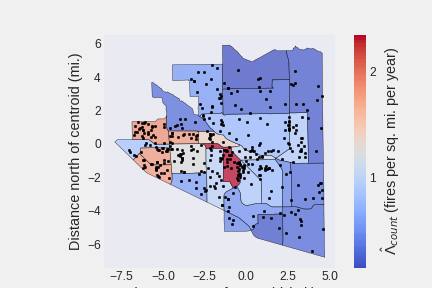
\includegraphics[width=.75\textwidth]{./figures/spatial_histogram.png}
\caption{A visual depiction of the naive count forecasting methodology for an example department. The black "x" markers each indicate the loction of a residiental fire that occurred during the six-year training interval, 2006-2011 (inclusive).}
\label{fig:spatial_histogram}
\end{figure}

\subsubsection{Kernel density estimation}
The second spatial model discussed in this paper is Kernel density estimation (KDE), which is a statistical methodology for inferring a density distribution from a set of point observations. This is the framework commonly used to generate incident heatmaps. The major difference between this method and the one outlined in the previous section is that is generates a smoothed surface that does not arise from ''binning" the incidents into discrete areas such as the census tract boundaries. Instead, this density surface is generated by centering a kernel function on each point (i.e. residential fire location) in the training set. The density function can then be calculated at any location by summing the kernel functions of all points at that location. This approach is illustrated in Figure ___. In order to provide intuition, a one dimensional example is also shown in addition to an example depicting the residential fire density for a department in the dataset. 











\clearpage
\bibliographystyle{unsrtnat}
\bibliography{./papers/references}
\end{document}
